% This template was initially provided by Dulip Withanage.
% Modifications for the database systems research group
% were made by Conny Junghans,  Jannik Strötgen and Michael Gertz

% Further modification based on Scientific Computing Master Thesis Template

\documentclass [
     12pt,         % font size
     a4paper,      % paper format
     BCOR10mm,     % binding correction
     DIV14,        % stripe size for margin calculation
     liststotoc,   % table listing in toc
     bibtotoc,     % bibliography in toc
     idxtotoc,     % index in toc
     parskip       % paragraph skip instad of paragraph indent
     ]{scrreprt}

%%%%%%%%%%%%%%%%%%%%%%%%%%%%%%%%%%%%%%%%%%%%%%%%%%%%%%%%%%%%

% PACKAGES:

% Use German/English :
%\usepackage[ngerman]{babel}
\usepackage[english]{babel}

% Input and font encoding
\usepackage[latin1]{inputenc}
\usepackage[T1]{fontenc}

% Index-generation
\usepackage{makeidx}
% Einbinden von URLs:
\usepackage{url}
% Special \LaTex symbols (e.g. \BibTeX):
\usepackage{doc}
% Include Graphic-files:
\usepackage{graphicx}
\usepackage{amssymb}

\usepackage{caption}
\usepackage{subcaption}
\usepackage{array}

% Include doc++ generated tex-files:
%\usepackage{docxx}
% Include PDF links
%\usepackage[pdftex, bookmarks=true]{hyperref}

% Fuer anderthalbzeiligen Textsatz
\usepackage{setspace}

% hyperrefs in the documents
\usepackage[bookmarks=true,colorlinks,pdfpagelabels,pdfstartview = FitH,bookmarksopen = true,bookmarksnumbered = true,linkcolor = black,plainpages = false,hypertexnames = false,citecolor = black,urlcolor=black]{hyperref} 
%\usepackage{hyperref}

% maths equations
\usepackage{amsmath}

\usepackage{listings}% http://ctan.org/pkg/listings

% paragraph indentation and spacing
\setlength{\parindent}{0em} 
\setlength{\parskip}{1.5em}

%%%%%%%%%%%%%%%%%%%%%%%%%%%%%%%%%%%%%%%%%%%%%%%%%%%%%%%%%%%%

% OTHER SETTINGS:

% Pagestyle:
\pagestyle{headings}

% Choose language
\newcommand{\setlang}[1]{\selectlanguage{#1}\nonfrenchspacing}


\begin{document}

% Title 
%% TITLE:
\pagenumbering{roman} 
\begin{titlepage}


\vspace*{1cm}
\begin{center}
\vspace*{3cm}
\textbf{ 
\Large Heidelberg University\\
\smallskip
\Large  Faculty of Mathematics and Computer Science\\
\smallskip
\Large  Institute of Computer Science\\
\smallskip
\Large Database Systems Research Group\\
\smallskip
}

\vspace{3cm}

\textbf{\large Master Thesis in Scientific Computing}  

\vspace{0.5\baselineskip}
{\huge
\textbf{Building a Map of Explicit Causal Factors from Financial Documents}
}

%%%% TO BE REMOVED BEFORE FINAL VERSION
\vspace{0cm}
----------------------------------------------------------------------------------------------
{\huge \textbf{[DRAFT as of \today] } }
----------------------------------------------------------------------------------------------
%%%% TO BE REMOVED BEFORE FINAL VERSION



\end{center}

\vfill 

{\large
\begin{tabular}[l]{ll}
Name: & Claire Zhao Sun\\
Matriculation Number: & 3630998\\
Supervisor: & Prof. Dr. Michael Gertz\\
Submission Date: & 2022.05.30
\end{tabular}
}

\end{titlepage}




%% Titleintro
%\thispagestyle{empty}
%\begin{center}
%  \renewcommand{\baselinestretch}{2.00}
% \Large\sffamily
%  Department of Mathematics and Computer Science\\
%  \large University of Heidelberg
%  \par\vfill\normalfont
%  Master thesis\\
%  in Scientific Computing\\
%  submitted by\\
%  (name and surname)\\
%  born in (place of birth)\\
%  (year of submission)
%\end{center}
%\newpage

%% Titlepage
%\thispagestyle{empty}
%\begin{center}
%  \renewcommand{\baselinestretch}{2.00}
%  \Large\bfseries\sffamily
%    (Title)\\
%    (of)\\
%    (Master thesis)
%  \par
%  \vfill
%  \large\normalfont
%  This master thesis has been carried out by (Name Surname)\\
%  at the\\
%  (institute)\\
%  under the supervision of\\
%  (Frau/Herrn Prof./Priv.-Doz. Name Surname)
  %% additionally insert second supervisor here if applicable
%\end{center}\par
%\vspace{5\baselineskip}

% reset baselinestretch
%\renewcommand{\baselinestretch}{1.00}\normalsize

% Declaration
%\setlength{\parindent}{0em}

Erkl\"{a}rung:\par
\vspace{2\baselineskip}
Ich versichere, dass ich diese Master-Arbeit selbstst\"{a}ndig verfasst und nur die angegebenen
Quellen und Hilfsmittel verwendet habe und die Grunds\"{a}tze und Empfehlungen "Verantwortung in der Wissenschaft" der Universit\"{a}t Heidelberg beachtet wurden. 

\vspace*{50pt}
\noindent

\underline{\phantom{mmmmmmmmmmmmmmmmmmmm}}

\medskip
\noindent
 
Abgabedatum: 2022.05.30





\vspace{10\baselineskip}

Declaration:\par
\vspace{2\baselineskip}
I hereby confirm that I wrote this Master Thesis independently and only used the specified sources, based on the principles and recommendations of "Responsibility in Science'' of Heidelberg University.
\par

\vspace*{50pt}
\noindent

\underline{\phantom{mmmmmmmmmmmmmmmmmmmm}}

\medskip
\noindent 
Submission Date: 2022.05.30



\newpage


% Add a brief summary of your topic and contributions (Zusammenfassung) in German *and* in English:
%\chapter*{Zusammenfassung}
%
% This file contains the German version of your abstract, with about 300-500 words

Die Zusammenfassung muss auf Deutsch \textbf{und} auf Englisch geschrieben
werden. Die Zusammenfassung sollte zwischen einer halben und einer
ganzen Seite lang sein. Sie soll den Kontext der Arbeit, die
Problemstellung, die Zielsetzung und die entwickelten Methoden sowie
Erkenntnisse bzw.~Ergebnisse �bersichtlich und verst�ndlich
beschreiben.
%\newpage

%\chapter*{Abstract}
%
% This file contains an abstract of your thesis, with approximaltely 300-500 words

The abstract has to be given in German \textbf{and} English. It should
be between half a page and one page in length. It should cover in a
readable and comprehensive style the context of the thesis, the
problem setting, the objectives, and the methods developed in this
thesis as well as key insights and results.

\newpage


% MAIN PART:
% Table of contents (Inhaltsverzeichnis)
\tableofcontents
\cleardoublepage
\pagenumbering{arabic} 

% List of figures (Abbildungsverzeichnis):
%\listoffigures
% List of tables (Tabellenverzeichnis):
%\listoftables


%%%%%%%%%%%%%%%%%%%%%%%%%%%%%%%%%%%%%%%%%%%%%%%%%%%%%%%%%%%%%%%
% Here, the actual content of your thesis begins
% You can either put all the text here or use individual files to store the chapters of your thesis.
% Below are templates for both alternatives.


%%%%%%%%%%%%%%%%%%%%%%%%%%%%%%%%%%%%%%%%%%%%%%%%%%%%%%%%%%%%

% TODO: better title
\chapter{Conceptual Framework} \label{conceptualization}

This chapter specifies the conceptual framework for a graph-based data model that represents the causal factors influencing the financial performance of S\&P 500 companies. Some general computational approaches for solving the problems stated in Chapter 1 are also provided. Section \ref{sec:overview} starts with an overview of the primary objectives of the data model, followed by a brief discussion of causal factor representation in Section \ref{sec:causalrepresenation}. In Section \ref{sec:datamodel}, a detailed description of the data model and a discussion of its main characteristics are presented. 
%Section \ref{sec:similarity} introduces similarity measures and algorithms to be performed on the data model. 


\section{Overview and Objectives} \label{sec:overview} 

As mentioned in Chapter 1, the primary motivation for this thesis is to create a text mining tool that mines financial reports to aid investment research. In practice, an important area of focus in investment research concerns companies' business models and underlying industry trends. Some specific questions that investment analysts need to address include:

\begin{itemize}
\item	What factors affect a particular company's financial performance? 
\item	How do these factors generally change over time? Are there any recognizable patterns?
\item  Which are the most closely related and comparable peers of a given company?
\item	Given certain macro-level events, e.g., geopolitical conflicts, food price inflation, interest rate hikes, etc., which companies are most likely to be affected?
\end{itemize}

For the purpose of this thesis, \emph{\textbf{causal factors}} are defined as a set of specific events, a general economic phenomenon, or a category of business activities, etc., which impact the financial performance of a company or a group of companies for a defined period of time. These causal factors necessarily cover a wide range in scope. They are allowed to be as specific or as general as possible. The intention of the flexibility in this definition is to enable capturing not only the immediate, direct drivers of key performance indicators (KPIs), but also general shifts in macro and sector trends that affect many companies over the long run. Examples of causal factors include: a pandemic such as COVID-19, wage increases, headcount changes, growth in paid subscriber base, etc..  

Understanding these causal factors helps investors forecast the future performance of companies under different scenarios to evaluate their intrinsic worth. Comparing a company's relative value with its peers in the same or related sectors can lead to investment opportunities such as the identification of undervalued companies and the early discovery of emerging themes and trends. 

Answers to most of these questions can be found in financial reports. However, they do not exist in a readily available form that can be directly retrieved via keyword search. These answers need to be synthesized through incorporation of relevant information, abstraction and summarization. When designing a system that can explicitly address these questions by mining information from financial reports, we gather inspiration from observing financial analysts' workflow and attempt to incorporate as much expert knowledge as possible in it. 

The \textbf{first observation} is that an experienced analyst usually knows where to look for relevant information in the financial reports. Instead of the most naive approach of reading them linearly in their entirety, he or she can quickly locate the specific sections to focus on, based on awareness of the report's structure and prior knowledge. Moreover, within the relevant section, an analyst also pays more attention to the sentences that explicitly express credit attribution in order to extract useful information. For example, a sentence such as \emph{"There was an increase in operating expenses primarily driven by an increase in compensation expenses largely due to increases in headcount."} is what the analyst would be focused on, if he or she is primarily interested in finding out what causal factors affect the \emph{operating expenses}. In this example sentence, the causal explanation associated with the effect of \emph{"increase in operating expenses"} can be attributed to the explicit factors such as \emph{"an increase in compensation expenses"} and \emph{"increases in headcount"}. We would like our system to incorporate these heuristic rules to facilitate the information extraction process.

The \textbf{second observation} is that people naturally process information through abstraction and categorization of similar concepts. Once a causal factor that affects the financial performance of a particular company is identified, the analyst is able to naturally associate it with similar causal factors of related companies. As they accumulate a wealth of associative knowledge throughout the years, they develop a sense about which companies are affected by certain causal factors and in what ways. Therefore, we need a representation of these causal factors which enables our system to perform similar tasks of abstraction and association. In other words, our system needs to be able to cluster these causal factors into meaningful groups that facilitate pattern discovery.

The \textbf{third observation} is the dynamic nature of and the interwoven complexity in the patterns of company-factor relations. We know from experience that some causal factors are company-specific, while others are generic and shared among many companies at the macro-level. In addition, some factors might be related to a one-off event, yet other times they could be recurring or cyclical in nature. Furthermore, it is also essential that the data model is capable of adapting to new patterns. The causal factors evolve with time, hence, the data model needs to be updated incrementally as new information becomes available.
  
To derive such a data model with these specific requirements, we need a two-staged approach. Firstly, all the causal factors are to be extracted from the raw texts of individual companies' financial reports. Next, the extracted factors are further processed via clustering algorithms. In addition, the data model should be accessible and queryable by users to retrieve data and output visualizations. Figure \ref{fig:pipeline} illustrates the envisioned data processing pipeline to achieve this purpose.  

\begin{figure}[h!]
\centering
  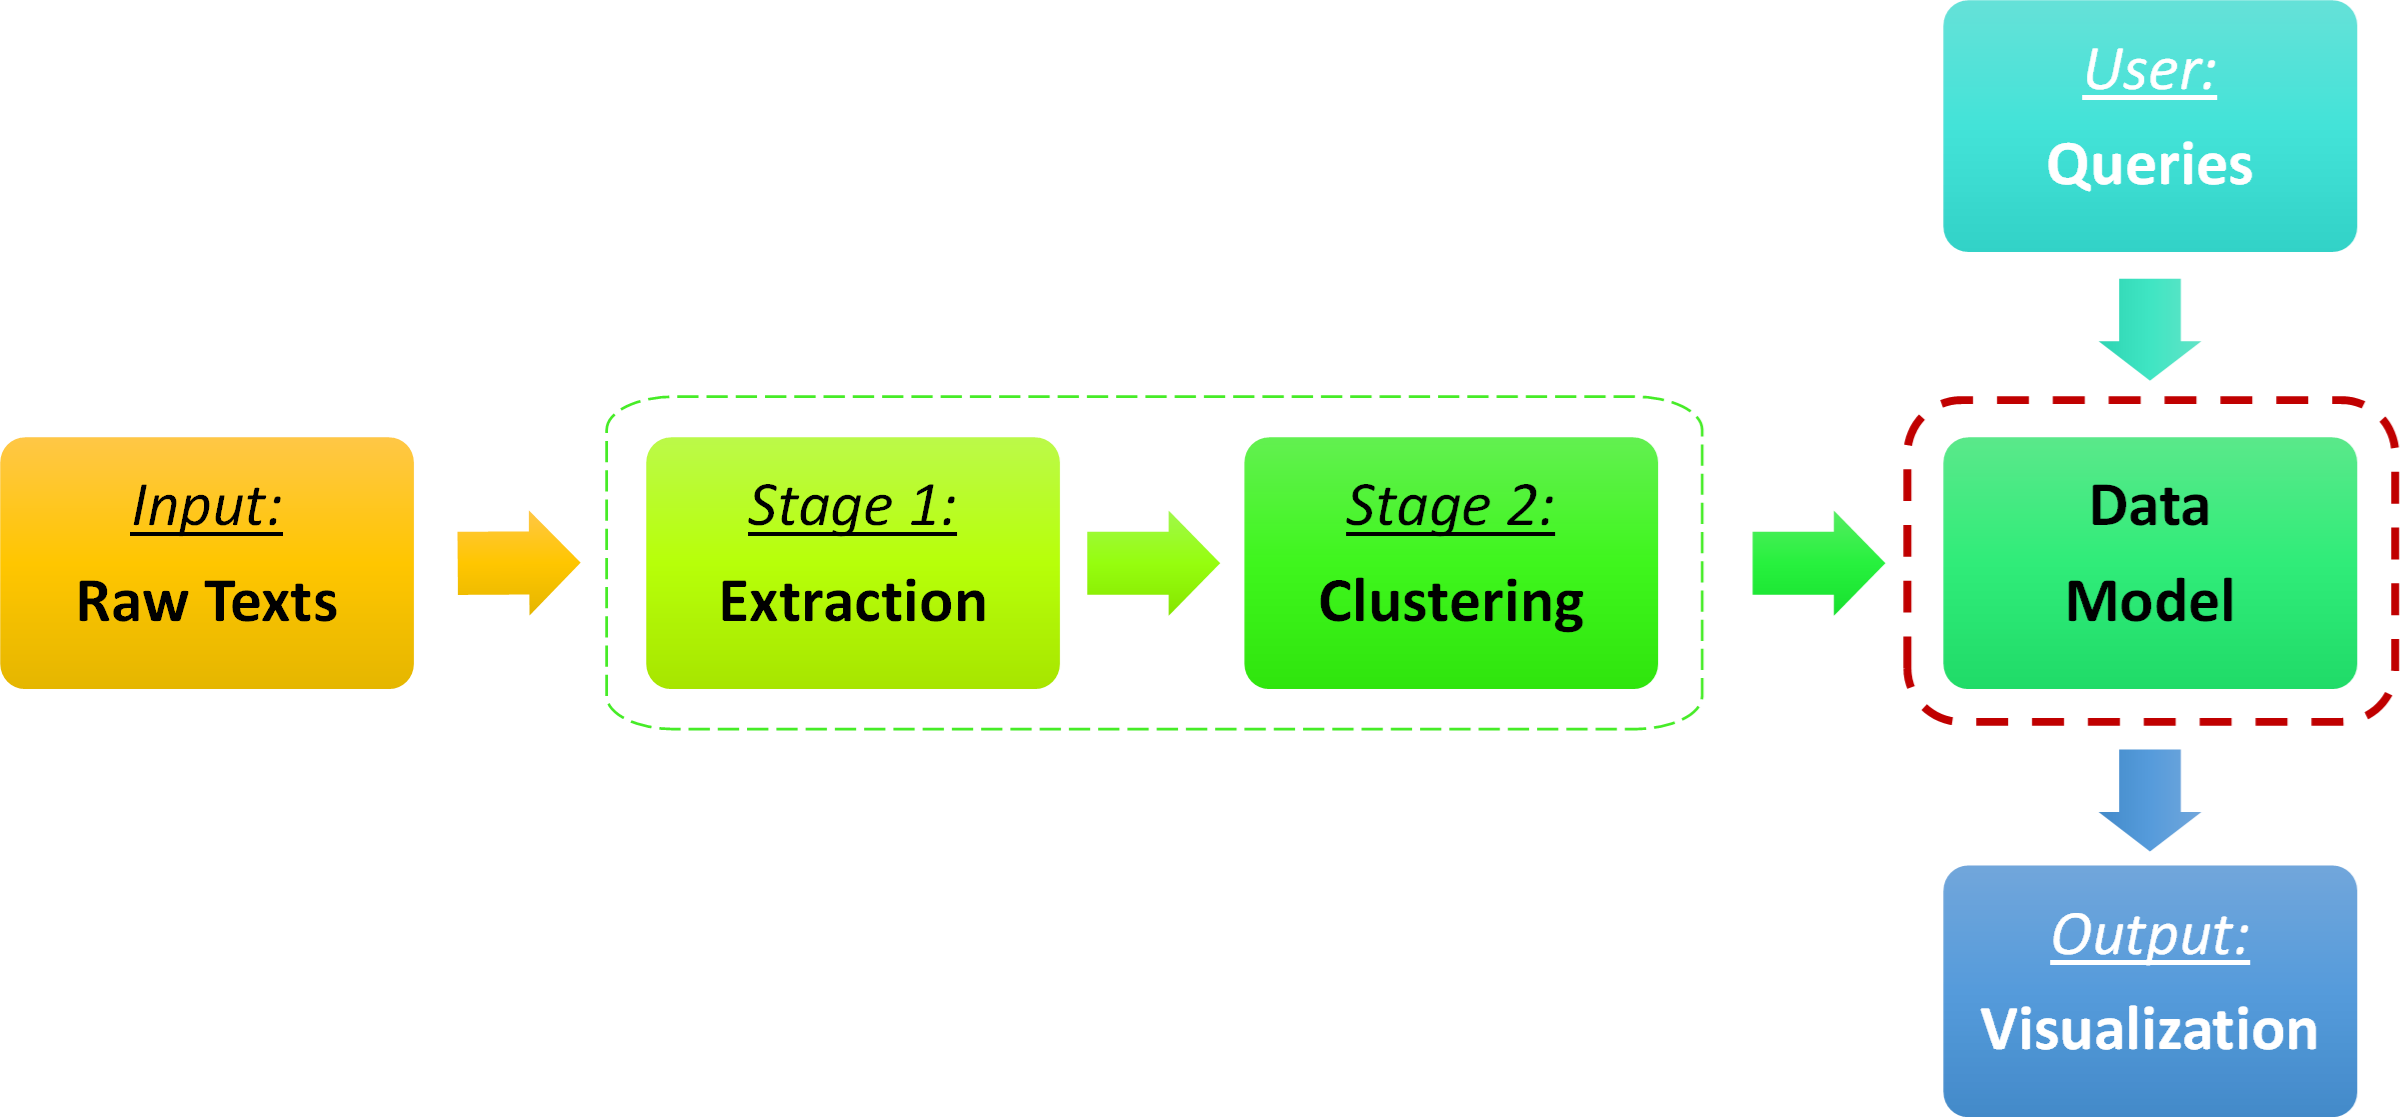
\includegraphics[scale=1.4]{figures/Pipeline_0.png}
  \caption{Illustration of Data Processing Pipeline}
  \label{fig:pipeline}
\end{figure}



\section{Definitions and Representations} \label{sec:causalrepresenation}

%TODO
In this section, we define \emph{causal sentences} and \emph{causal factors} in the context of our data model. We first establish a common understanding of causal sentences' structure patterns in terms of \emph{cause} and \emph{effect chunks}. We also introduce the concept of \emph{topics} in relation to causal sentences in financial reports. Finally, we define \emph{causal factors} and discuss their representation. 

\subsection{Causal Sentences}
In the data model, a \emph{\textbf{causal sentence}} is defined as a sentence that contains three components: a cause (C), an effect (E) and an explicit causal connector (CC). A cause is a text fragment within a sentence that describes an event or phenomenon that claims to cause another event or phenomenon, i.e., the effect. These cause and effect text fragments can be a word, a phrase or a clause. 

A causal connector is a linguistic signal of causality and it can appear in the form of a verb (e.g., E \emph{driven} by C), a prepositional phrase (e.g., E \emph{due to} C), a conjunction (e.g., E \emph{because} C), etc. It serves as a marker to segment a causal sentence into chunks of text fragments corresponding to cause and effect. For example, the causal sentence, \emph{"The increase in operating expenses was primarily driven by an increase in sales and marketing cost."}, can be represented as: E = \emph{"the increase in operating expenses"}, CC = \emph{"driven by"}, C = \emph{"an increase in sales and marketing cost"}. Any causal sentence can be represented as one of two patterns of cause-effect chunks linked by causal connectors, as illustrated by Figure \ref{fig:blockpatterns} (a) and (b).  

Depending on the causal connector's part-of-speech function, as well as the complexity of the corresponding cause and effect chunks, the causal sentence can have a simple, compound or complex sentence structure. For example, a causal sentence such as \emph{"Growth for our direct response advertising products was primarily driven by increased advertiser spending as well as improvements to ad formats and delivery."}, contains multiple causes, C1 =\emph{"increased advertiser spending"} and C2 =\emph{"improvements to ad formats and delivery"}, attributed to one single effect, E = \emph{"Growth for our direct response advertising products"}. In this case, the data model treats C1 and C2 as one combined cause chunk. See illustration in Figure \ref{fig:blockpatterns} (c).

As another example, in the sentence \emph{"There was an increase in operating expenses primarily driven by an increase in compensation expenses largely due to increases in headcount"}, there is a causal chain with multiple causal connectors (\emph{"driven by", "due to"}). In theory, this causal sentence can be broken down into two subsets of cause and effect chunks: 1) E1 = \emph{an increase in operating expenses}, C1 = \emph{an increase in compensation expenses}; 2) E2 = \emph{an increase in compensation expenses}, C2 = \emph{increases in headcount}, where E2 = C1. In this case, the data model treats C1 and C2 as a combined cause chunk, as illustrated in Figure \ref{fig:blockpatterns} (d).  


\begin{figure}[h!]
\centering
  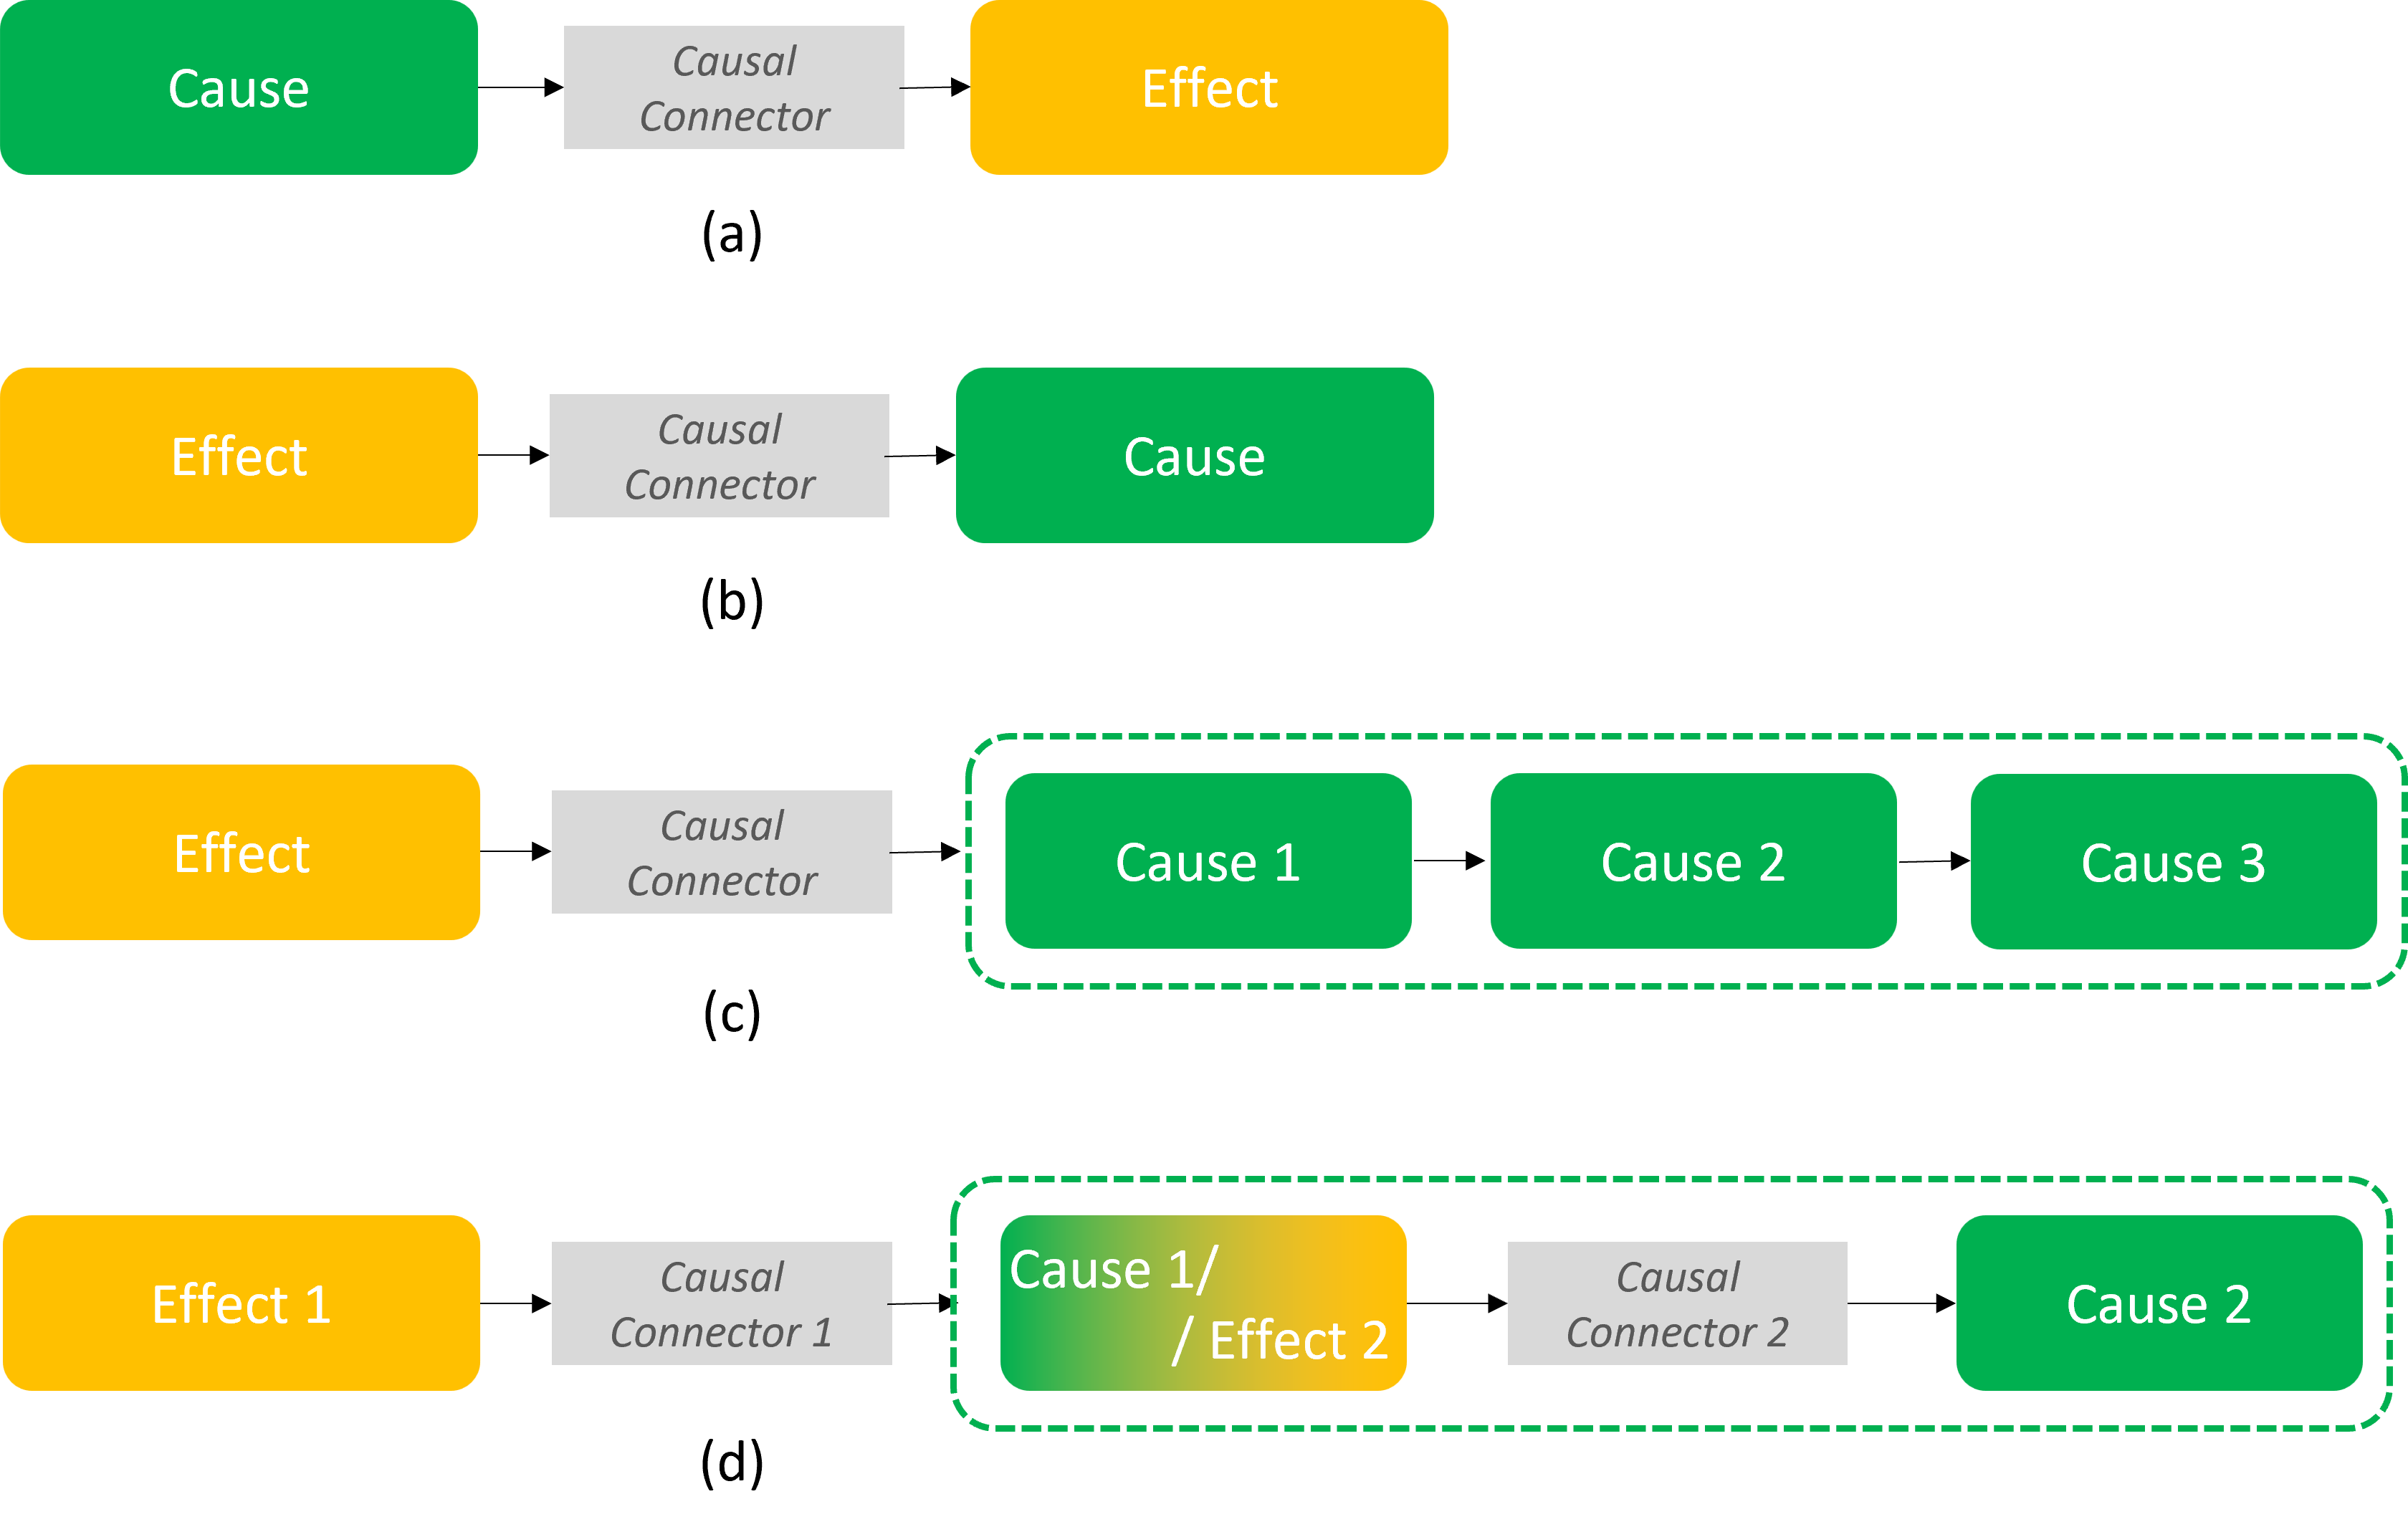
\includegraphics[scale=0.5]{figures/CausalBlocks.png}
  \caption{Illustration of typical patterns in causal sentences. (a) and (b) are patterns of simple causal sentences involving only one cause and one effect. (c) represents a compound causal sentence with one effect and multiple causes. (d) represents a compound causal sentence with two causal connectors. In both cases (c) and (d), the data model treats the complex causes as a combined chunk.}
  \label{fig:blockpatterns}
\end{figure}



%[justification for this simplification]. 
In the context of financial reports, management explains about a company's performance in a formal business language that is logical, concise and unambiguous. Causal sentences typically have an effect chunk referring to a change in one particular financial metric, for example, growth in \emph{revenue}, decline in \emph{gross profit}, improvement in \emph{earnings before interest, tax, depreciation and amortization (EBITDA) margin}, decrease in \emph{net income}, etc. Accordingly, a \emph{\textbf{topic}} is defined as a financial metric term that is expressed in an effect chunk of a causal sentence. Specifically, the \emph{topics} referred to in the above examples are \emph{revenue, gross profit, EBITDA margin} and \emph{net income}.


\subsection{Causal Factors}

The cause chunk in a causal sentence typically expresses the explanation of factors that affect a business' financial performance. In our data model, these factors are referred to as \emph{\textbf{causal factors}} (see definition in Section \ref{sec:overview}). Theoretically, there are many possible ways of representing these causal factors. 

The most naive way is to treat each cause chunk as one cause factor and store the original text fragments in a database which can be searched via key words. To compare similarities amongst these factors, a bag-of-words or TFIDF approach could be applied. However, the key limitations of this approach is that it ignores the structure and semantic information embedded in text fragments and the weight of each term only reflects the term frequency rather than the functional role in a sentence. In addition, the size of vocabulary as the dimension of the vector representation resulting in sparse data in a high-dimensional space, which is computationally inefficient to deal with.  

Another approach is to represent these factors as events with a template specifying a set of pre-defined features, such as time, location, actor, movement, etc. The advantage is to have a controllable number of features. However, this slot-filling approach requires a lot of expert input in order to manually handcraft. The factors could be diverse and therefore difficult to design a template that fits all scenarios.   

Taking inspiration from both of the above mentioned methods, we adopt the following approach: a cause chunk is represented as a directed graph, where the vertices are the noun phrases in the text fragment and the directed edges represents the connecting texts that are in between those noun phrases. The connecting text could be a verb, a conjunction, part of a preposition phrase, etc.. 

In this model, the noun phrases are treated as carriers of concepts and the connection texts as indication of relationships between these concepts. These noun phrases are further clustered into groups based on semantic similarities. In other words, we group synonyms or phrases representing similar concepts into the same cluster. Ideally, a concept can be identified from each cluster of noun phrases. These clusters can also be considered as equivalent to the slots in a template, except these features are automatically generated based on unsupervised learning rather than manually defined by expert beforehand. 

Replacing each noun phrase with its corresponding concept cluster that it belongs to, each cause chunk can therefore be represented as a sequence of connected concept clusters in the direct graph. Instead of using each unique noun phrase as a feature, we use these concept clusters as feature space, thus effectively reducing the dimensionality of feature space to represent these factors. 

Alternatively, we could use a language model such as BERT to obtain the contextualized embeddings for these text fragments, however, this black-box approach is not interpretable. 




\section{Data Model} \label{sec:datamodel}

In this section, we describe our data model in details. We first establish the data model as a heterogenous graph, then elaborate on the specification for each node type and how the data model is built step by step. We also discuss the key characteristics of the data model. 

\subsection{Node and Edges}

In essence, our data model is a heterogeneous graph $\mathbf{G} = (\mathbf{V}, \mathbf{E})$ with five distinct node types: \emph{Company}, \emph{Document}, \emph{CausalSentence}, \emph{NounPhrase}, and \emph{Concept}.
\[\mathbf{V} = \mathbf{V}_{company} \cup \mathbf{V}_{document} \cup \mathbf{V}_{causalSentence} \cup \mathbf{V}_{nounPhrase} \cup \mathbf{V}_{concept} \]

There exists a natural order of hierarchy among these nodes, which is indicated by the four distinct types of directed edges:
\[\mathbf{E} = \mathbf{E}_1 \cup \mathbf{E}_2 \cup \mathbf{E}_3 \cup \mathbf{E}_4 \] where 
\[\mathbf{E}_1 \subseteq \mathbf{V}_{company} \times \mathbf{V}_{document} \]
\[\mathbf{E}_2 \subseteq \mathbf{V}_{document} \times \mathbf{V}_{causalSentence} \]
\[\mathbf{E}_3 \subseteq \mathbf{V}_{causalSentence} \times \mathbf{V}_{nounPhrase} \]
\[\mathbf{E}_4 \subseteq \mathbf{V}_{nounPhrase} \times \mathbf{V}_{concept} \]


We now elaborate on the specification for each node type and the associated edges. We use $(...)$ to denote \emph{nodes}, $-[...]\rightarrow$ to denote \emph{edges} and \{...\} to denote edge properties.


\paragraph{Company Nodes:} Company nodes ($\mathbf{V}_{company}$) represent a set of companies, $\mathcal{C}$, where $\mathbf{V}_{company} \subseteq \mathbf{\mathcal{C}}$. Each company node is identifiable by a unique ticker. Additional node properties include the company's full name and its sector classification. For example, Alphabet Inc. is represented as a company node with the ticker \emph{GOOGL}, company name \emph{Alphabet Inc.} and sector classification \emph{Communication Services}.  


\paragraph{Document Nodes:} Document nodes ($\mathbf{V}_{document}$) represent a set of financial documents, $\mathbf{\mathcal{D}}$, where $\mathbf{V}_{document} \subseteq \mathbf{\mathcal{D}}$. In our case, the set of financial documents consist of form 10-Qs and 10-Ks (see Section 2.3.1). Each financial document is associated with a particular company identifiable by the same unique ticker, as well as a $timestamp$ corresponding to the document's reporting period.  


\paragraph{Directed Edge from Company Nodes to Document Nodes:} There is a one-to-many relationship from the company set to the document set. Each company can be associated with multiple documents over an extended period of time, whereas each document can only be associated with one company. The company-document relationship is represented by a directed edge, $\mathbf{E}_1 \subseteq \mathbf{V}_{company} \times \mathbf{V}_{document}$, in the graph. For each edge, the $timestamp$ encoding the document's reporting period is specified as an edge property, as illustrated below:
\[( c_i ) - [ e_1 \{timestamp\} ]\rightarrow ( d_j ) \]
where $c_i \in \mathbf{V}_{company}$,  $d_j \in \mathbf{V}_{document}$ and $e_1 \in \mathbf{E}_1$.


\paragraph{CausalSentence Nodes:} CausalSentence nodes ($\mathbf{V}_{causalSentence}$) represent a set of sentences which express causality, $\mathbf{\mathcal{S}}$, where $\mathbf{V}_{causalSentence} \subseteq \mathcal{S}$. In our case, the set of causal sentences are extracted from the set of financial documents $\mathbf{\mathcal{D}}$ through a mapping: 
\[f_{extract-causal}: \mathbf{\mathcal{D}} \rightarrow \mathbf{\mathcal{S}}\] 
where $f_{extract-causal}$ corresponds to the process of extracting causal sentences from the set of financial documents.

As discussed in Section 3.2, causal sentences can be decomposed into cause and effect chunks, and the effect chunks typically describe changes or movements in some financial metrics, such as increase in revenue, decrease in margins, and increase in net income. Therefore each causal sentence can be tagged with a $topic$ which refers to the underlying financial metric reflected in the effect chunk. The typical $topics$ include the most common financial Key Performance Indicators (KPIs) such as: \emph{revenue (or sale), cost (or expense), income (or profit), earnings before interest and taxt (EBIT), gross margin, net margin, etc.}. 


\paragraph{Directed Edge from Document Nodes to CausalSentence Nodes:} There is also a one-to-many relationship from the document set to the causalSentence set, since each causal sentence is only associated with one document but multiple causal sentences can be extracted from the same document. The document-causalSentence relationship is represented by a directed edge, $\mathbf{E}_2 \subseteq \mathbf{V}_{document} \times \mathbf{V}_{causalSentence}$, in the graph. For each edge, the $topic$ identified from the effect chunk of the causal sentence, is listed as an edge property, as illustrated below:
\[( d_j ) - [ e_2 \{topic\} ]\rightarrow ( s_k ) \] 
where $d_j \in \mathbf{V}_{document}$, $s_k \in \mathbf{V}_{causalSentence}$ and $e_2 \in \mathbf{E}_2$.


\paragraph{NounPhrase Nodes:} NounPhrase nodes ($\mathbf{V}_{nounPhrase}$) represent a set of noun phrases, $\mathbf{\mathcal{N}}$, where $\mathbf{V}_{nounPhrase} \subseteq \mathcal{N}$. In our case, the set of noun phrases are extracted from the set of causal sentences $\mathbf{\mathcal{S}}$ through a mapping: 
\[f_{extract-np}: \mathbf{\mathcal{S}} \rightarrow \mathbf{\mathcal{N}}\] 
where $f_{extract-np}$ represents the process of extracting noun phrases from the cause chunks of the causal sentences, as discussed in Section 3.2. For example, the causal sentence \emph{"The increase was primarily driven by <high levels of promotional expense in the first quarter of fiscal 2015, a decrease in SG\&A expenses, and lower supply chain costs>."} contains a cause chunk marked in <...>. This cause chunk can be further segmented into the following noun phrases and represented in an ordered list:
[1. \emph{high levels}, 2. \emph{promotional expense}, 3. \emph{the first quarter}, 4. \emph{a decrease}, 5. \emph{SG\&A expense}, 6. \emph{lower supply chain costs}]
The rational for choosing noun phrases, rather than other part-of-speech terms such as verbs, adjectives, etc., is based on the assumption that noun phrases are the most fundamental symbolic representation of concrete objects as well as abstract ideas, thus a natural choice for the basic lexical unit of concepts.


\paragraph{Directed Edge from CausalSentence Nodes to NounPhrase Nodes:} There is a many-to-many relationship between the causal sentence set and the noun phrase set. A causal sentence can contain multiple noun phrases and a noun phrase can be contained in multiple causal sentences. In addition, the order of the sequence that the noun phrase appear in a causal sentence is also important and must be encoded in the respective relationship. For the same example above, the edge connecting the noun phrase node \emph{high levels} to the sentence node should an $order$ value of 1; the edge associated with \emph{promotional expense} has an $order$ value of 2, etc. and so on for the rest of the nouns in the ordered list. 

Therefore, the relationships from the causal sentence to each of its constituent noun phrases are represented as directed edges, $\mathbf{E}_3 \subseteq \mathbf{V}_{causalSentence} \times \mathbf{V}_{nounPhrase}$. Each edge has a property that corresponds to the $order$ of the noun phrase's appearance in the cause chunk of the causal sentence, as illustrated below:
\[( s_k ) - [ e_3 \{order\} ]\rightarrow ( n_p ) \] 
where $s_k \in \mathbf{V}_{causalSentence}$, $n_p \in \mathbf{V}_{nounPhrase}$ and $e_3 \in \mathbf{E}_3$.


\paragraph{Concept Nodes:} Concept nodes ($\mathbf{V}_{concept}$) represent a set of concepts, $\mathbf{\mathcal{CC}}$, where $\mathbf{V}_{concept} \subseteq \mathcal{CC}$. A $concept$ is defined as an abstract representation of a group of semantically similar noun phrases. In this case, the set of concepts are formed from partitioning the set of noun phrases into a set of clusters, with each cluster representing a concept
\[f_{cluster-np}: \mathbf{\mathcal{N}} \rightarrow \mathbf{\mathcal{CC}}\] 
where $f_{cluster-np}$ represents the hard clustering process of assigning each noun phrase to one particular concept. For example, noun phrases such as \emph{Europe, EU, Middle East, Africa, Asia Pacific, North Americas}, etc. are expected to form a cluster, from which the concept of \emph{continent or region} can be identified.  


\paragraph{Directed Edge from NounPhrase Nodes to Concept Nodes:} There is a many-to-one relationship between the noun phrase set and the concept set. This results directly from the condition of hard clustering: each concept consists of multiple noun phrases, however, each noun phrase can only be clustered into one concept. The relationships between the noun phrase sets and the concept sets are represented by directed edges, $\mathbf{E}_4 \subseteq \mathbf{V}_{nounPhrase} \times \mathbf{V}_{concept}$, in the graph:
\[( n_p ) - [ e_4 \{order\} ]\rightarrow ( cc_q ) \] 
where $n_p \in \mathbf{V}_{nounPhrase}$, $cc_q \in \mathbf{V}_{concept}$ and $e_4 \in \mathbf{E}_4$.
There is a potential to extend this model to soft clustering where the edge can also encode the probability. However, this is beyond the scope of this thesis. 


Figure \ref{fig:AssumpSet} provides a graphical overview of the set relationships among the five distinct node types in the heterogenous graph-based data model.
\begin{figure}[h!]
\centering
  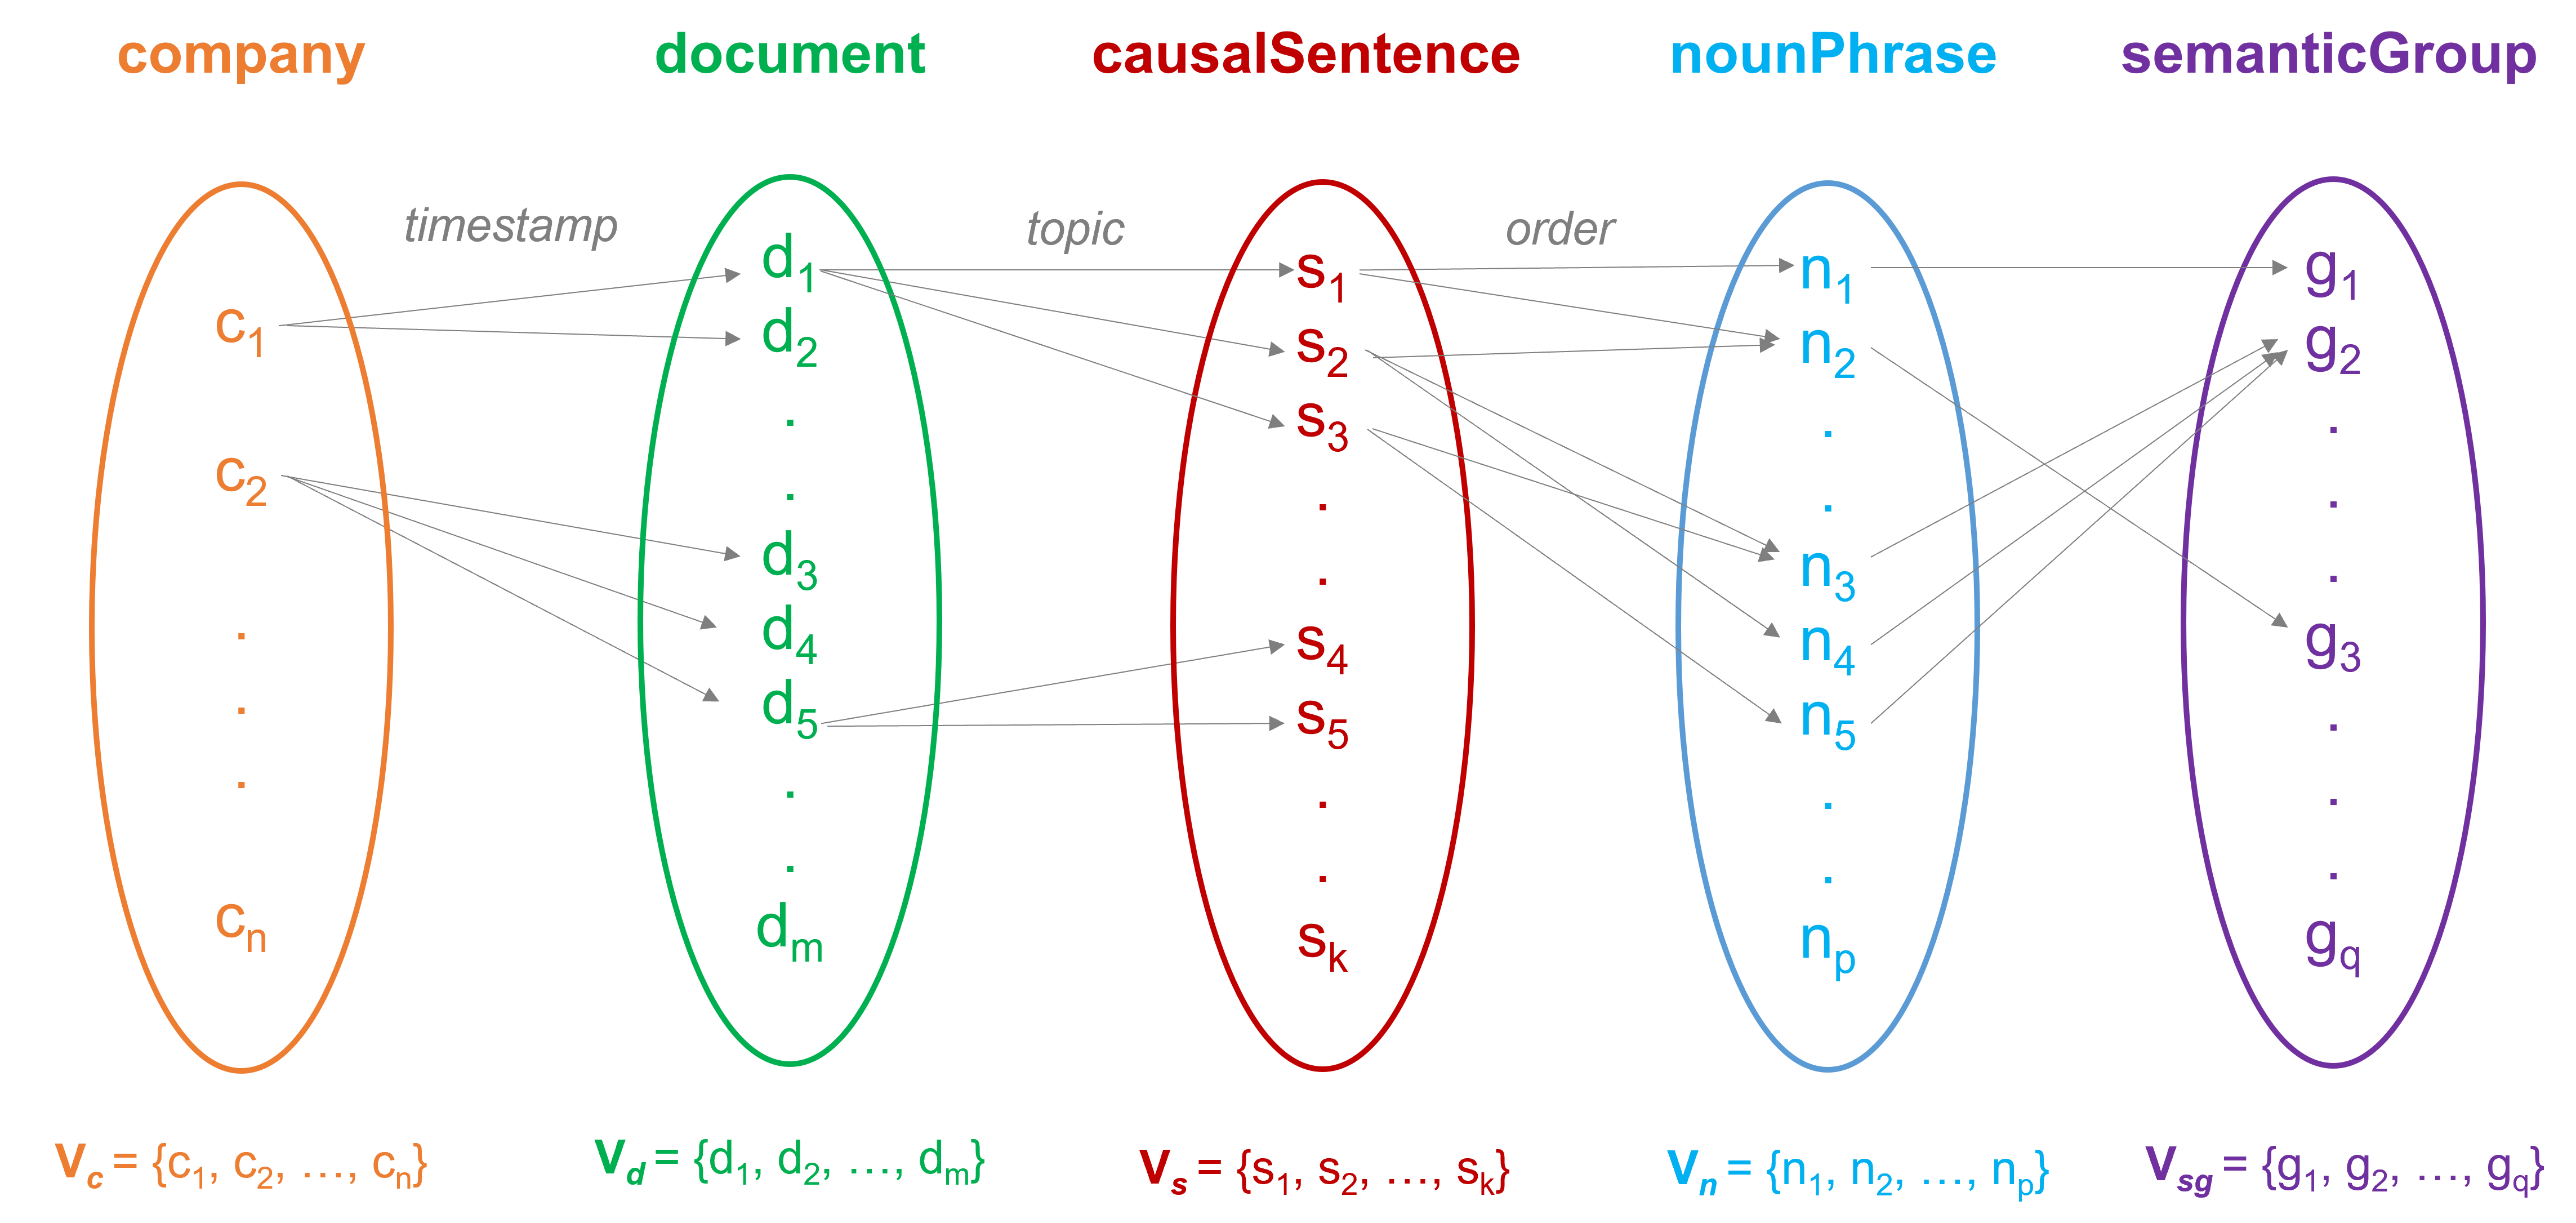
\includegraphics[scale=0.4]{figures/Sets.png}
  \caption{Illustration of set relationships among the company set, document set, causalSentence set, nounPhrase set and concept set.}
  \label{fig:AssumpSet}
\end{figure}

The primary goal of breaking the causal clauses into noun phrases is to transform the data model into a high dimensional latent space, where each specific cause is decomposed into individual features or latent factors. The primary goal of clustering noun phrases into concepts is to detect the hidden patterns and reduce the dimensionality of the sparse latent space. This effectively achieves data compression for generalization and data association in order to facilitate data retrieval. In addition, these concept clusters also enable direct connections to be made between companies which might be affected by implicitly similar factors that are semantically close in the latent space, but not expressed by exactly the same causal clauses at the explicit level. 

In summary, our data model has the following characteristics: 

\begin{itemize}
	\item	 It is a heterogeneous graph with five distinct types of nodes: \emph{Company, Document, CausalSentence, NounPhrase, and ConceptCluster}.
	\item	 These nodes follow a natural hierarchical order: \emph{Company $\rightarrow$ Document $\rightarrow$  CausalSentence $\rightarrow$ NounPhrase $\rightarrow$ ConceptCluster} 
	\item 	Concept nodes can be perceived as the connection points providing the means for similarity measures at different node levels. 
	\item 	Temporal information included in the graph make it possible to treat it as a dynamic graph, where an evolution of trends can be observed with respect to the passage of time. 
	\item 	The data model can be incrementally updated, when new financial reports become available.
\end{itemize}




%%%

\subsection{Node Embeddings and Similarity Measures} \label{sec:similarity}

Having established the basics of the data model, we now move on to define node embeddings and similarity measures between nodes. This paves the foundation for directly addressing the two objectives stated earlier in Section 3.1: the identification of performance drivers and the discovery of similar companies. Node embeddings and similarity measures are defined according to their respective node types.


% NounPhrase
\paragraph{NounPhrase Node Embedding:} Since a $NounPhrase$ node represents a noun or a noun phrase, the underlying word embedding is a natural choice for the node embedding. Different types of word embeddings, such as word2vec, GloVe and BERT, have already been discussed in Section 2.2.1. In addition, the various methods for computing phrase represenations from word vectors have also been discussed in Section 2.2.2. A suitable choice for the noun phrase node embeddings in our data model is a static word-level embedding model pre-trained on a relatively large corpora, such as pretrained GloVe embeddings. A simple average operation is opted for obtaining the compositional phrase embeddings from the constituents word embeddings. 
\[ \mathbf{Embedding}(NounPhrase) = \frac{1}{n} \sum_{i=1} ^n {\mathbf{w_i}}\]  
where $\mathbf{w_i}$ is the word embedding for the $i^{th}$ token in the $NounPhrase$ and $n$ is the total number of tokens in the $NounPhrase$. 

The similarity between a pair of $NounPhrase$ nodes is defined as the cosine similarity between the node embeddings. 
\[ \mathbf{Similarity}(NounPhrase_A, NounPhrase_B) = \frac{\mathbf{A \cdot B} } {\mathbf{\lVert A \rVert \cdot \lVert B \rVert}} \]  where $\mathbf{A}$ = \textbf{Embedding}($NounPhrase_A$), $\mathbf{B}$ = \textbf{Embedding}($NounPhrase_B$).

These similarity measures allows the grouping together of noun phrases which are closely related in semantics, while spacing wider apart the ones which are distantly related. These node embeddings are used as input to the clustering algorithm which generate $Concept$ nodes.

% Concept
\paragraph{Concept Node Embedding:} A $Concept$ node is effectively the centroid of the clusters of $NounPhrase$ nodes which are directly connected to it in the graph. The node embedding for a $Concept$ node is defined as:
\[ \mathbf{Embedding}(Concept) = \frac{1}{m} \sum_{j=1} ^n {\mathbf{V_j}}\] 
where $\mathbf{V_j}$ is the node embedding for the $j^{th}$ $NounPhrase$ in the immediate neighborhood of the $Concept$ node and $m$ is the total number of $NounPhrase$ nodes in the neighbourhood. 

The similarity between a pair of $Concept$ nodes is defined as the cosine similarity between the node embeddings. 
\[ \mathbf{Similarity}(Concept_X, Concept_Y) = \frac{\mathbf{X \cdot Y} } {\mathbf{\lVert X \rVert \cdot \lVert Y \rVert}} \]  where $\mathbf{X}$ = \textbf{Embedding}($Concept_X$), $\mathbf{Y}$ = \textbf{Embedding}($Concept_Y$).


% CasualSentence
\paragraph{CausalSentence Node Embedding:} Each $CausalSentence$ node is connected to an ordered set of $NounPhrase$ nodes that represent the constituent underlying noun phrases according to their order of appearance in the cause chunk of the sentence. Each $NounPhrase$ node is in turn connected to a $Concept$ node. Therefore, the node embedding for a $CausalSentence$ node can be represented as a list of $Concept$ node indices: 
\[ \mathbf{Embedding}(CausalSentence) = [cc_1, cc_2, ..., cc_i, ..., cc_n] \]
where $cc_i$ is the index of the $Concept$ node linked to the $NounPhrase$ node, which is connected to the $CausalSentence$ node with an edge order = $i$; $n$ is the total number of $NounPhrase$ nodes connected to the $CausalSentence$ node. 

The $CausalSentence$ node embeddings are allowed to have different lengths according to how many $NounPhrase$ nodes there are in its neighborhood. In other words, the lengths of the node embeddings also encode the amount of information content in the sentences represented by the $CausalSentence$ nodes. 

The similarity between a pair of $CausalSentence$ nodes is measured at two levels: weak similarity and strong similarity. The weak similarity is defined as the Jaccard similarity between the two node embeddings of the $CausalSentence$ nodes:
\[ \mathbf{Similarity}(CausalSentence_A, CausalSentence_B) = \frac{\| \mathbf{A \cap B} \|}{\|\mathbf{A \cup B} \|} \]  
where $\mathbf{A}$ = \textbf{Embedding}($CausalSentence_A$), $\mathbf{B}$ = \textbf{Embedding}($CausalSentence_B$).

Only if the weak similarity between two $CausalSentence$ nodes are above a certain threshold, then the strong similarity is defined. The strong similarity is used as a more precise measure of how similar the pair of nodes are when they are already considered somewhat similar by the weak similarity measure. If the pair of nodes has a weak similarity below the threshold, for example, when the pair of $CausalSentence$ nodes do not share any $Concept$ nodes in common, there is no practical need to further compute the strong similarity score between them. 

There are various methods to define the strong similarity, such as Levenshtein distance \cite{similarity2020} or Sorenseon-Dice coefficient \cite{similarity2020} based on the $CausalSentence$ node embeddings; alternatively, a cosine similarity between the sentence embeddings of the underlying text can be obtained from a pretrained model such as Sentence-BERT \cite{sentenceBERT2019}. The precision required for the strong similarity measure depends on the end application and how much computational resources are available in practice. The exploration in this regard is left to future studies. 

For the purpose of this thesis, only the weak similarity measure is applied, as there is no practical need to compare two individual sentences in the end application. 


% Document
\paragraph{Document Node Embedding:} Each $Document$ node is connected to a set of $CausalSentence$ nodes via edges labelled with $topics$, which are financial KPIs explained by the causal sentences. Accordingly, the $Document$ node embedding is defined as the collection of different sets of the $CausalSentence$ node embeddings, where $CausalSentence$ notes in each set correspond to a distinct $topic$. 
\[ \mathbf{Embedding}(Document) =  \{ \mathbf{D_t} \mid t \in topics(Document) \} \]
where
\[ \mathbf{D_t} = \{ \mathbf{Embedding}(CausalSentence_i) \mid CausalSentence_i \in \mathcal{N}_t(Document) \} \]
and $\mathbf{D_t}$ represents a set of $CausalSentence$ node embeddings under a topic $t$, $topics(Document)$ represents the set of $topics$ on the outgoing edges of the $Document$ node, $\mathcal{N}_t(Document)$ represents the set of $CausalSentence_i$ nodes in the immediate neighborhood of the $Document$ node under the topic $t$.

Equivalently, each $Document$ node embedding can be expressed in the form of a matrix, where each column is a vector representation of the distribution of the $Concept$ nodes under a $topic$. The dimension of the column vector is equal to the total number of unique $Concept$ nodes and each entry in the embedding corresponds to the number of counts for each $Concept$ node.
\[ \mathbf{Embedding}(Document) =  (d_{i,j}) \in \mathbb{R}^{m \times n} \] 
where $m=\mid \mathbf{V}_{Concept} \mid$,  $n=\mid \mathbf{E}_2 \mid$.

The similarity measure between two $Document$ nodes is defined as the cosine similarities of each pair of corresponding column vectors of the two nodes embedding matrices. The resulting representation is a row vector with each entry representing the similarity measure for each topic.
\[ \mathbf{Similarity}(Document_A, Document_B) = [ \mathbf{s_j} ] \in \mathbb{R}^{1 \times n}\]
\[  \mathbf{s_j} = \frac{\mathbf{a_j \cdot b_j} } {\mathbf{\lVert a_j \rVert \cdot \lVert b_j \rVert}} \]  
where 
\[ \mathbf{a_j} = \textbf{Embedding}(Document_A)[: , j] \]
and 
\[ \mathbf{b_j} = \textbf{Embedding}(Document_B)[: , j] \]


% Company
\paragraph{Company Node Embedding:} Each $Company$ node is connected to a set of $Document$ nodes through timestamped edges. A $Company$ node embedding is therefore represented as a tensor, i.e., a stack of $Document$ embedding matrices each representing a discrete timestamp. This approach naturally supports generating dynamic $Company$ node embeddings based on the specification of $time periods$ according to the use cases. 
\[ \mathbf{Embedding}(Company_{t_1}^{t_2}) = \sum_{t=t_1} ^{t=t_2} {\mathbf{Embedding}(Document_t)}\]  
where $Document_t \in \mathcal{N}_t(Company)$, the neighborhood of the $Company$ node for the specified period from $t=t_1$ to $t=t_2$. 

For a specified time period, the three-dimensional tensor representations of a $Company$ node embedding can be effectively transformed into a two-dimensional matrix by aggregating along the temporal axis by summation; the resulting matrix representation is effectively in the same form as a $Document$ node embedding as described above. 

The similarity measure between two $Company$ nodes, $(Company_A)_{t_1}^{t_2}$ for the time period from $t1$ to $t2$ and $(Company_B)_{\tau_1}^{\tau_2}$ for the time period from ${\tau_1}$ to ${\tau_2}$, are defined the cosine similarities of each pair of corresponding column vectors of the two nodes embedding matrices:
\[ \mathbf{Similarity}((Company_A)_{t_1}^{t_2}, (Company_B)_{\tau_1}^{\tau_2}) = [ \mathbf{s_j} ] \in \mathbb{R}^{1 \times n}\]
\[  \mathbf{s_j} = \frac{\mathbf{a_j^{T} \cdot b_j^{\mathcal{T}}} } {\mathbf{\lVert a_j^{T} \rVert \cdot \lVert b_j^{\mathcal{T}} \rVert}} \] 
where 
\[\mathbf{a_j^{T}} = \textbf{Embedding}((Company_A)_{t_1}^{t_2})[: , j] \] 
and
\[\mathbf{b_j^{\mathcal{T}}} = \textbf{Embedding}((Company_B)_{\tau_1}^{\tau_2})[: , j] \]

This approach not only allows the optional tracking of the temporal evolution of the $Company$ node embeddings at various granularity levels, e.g., quarterly, annually or every five years, but also enables comparison of companies across different periods of time. 




%\appendix
%\chapter {Appendix}
%\section{Papers on Causality Extraction}
\label{appendix:CEpapers}

\begin{figure}[h!]
\centering
  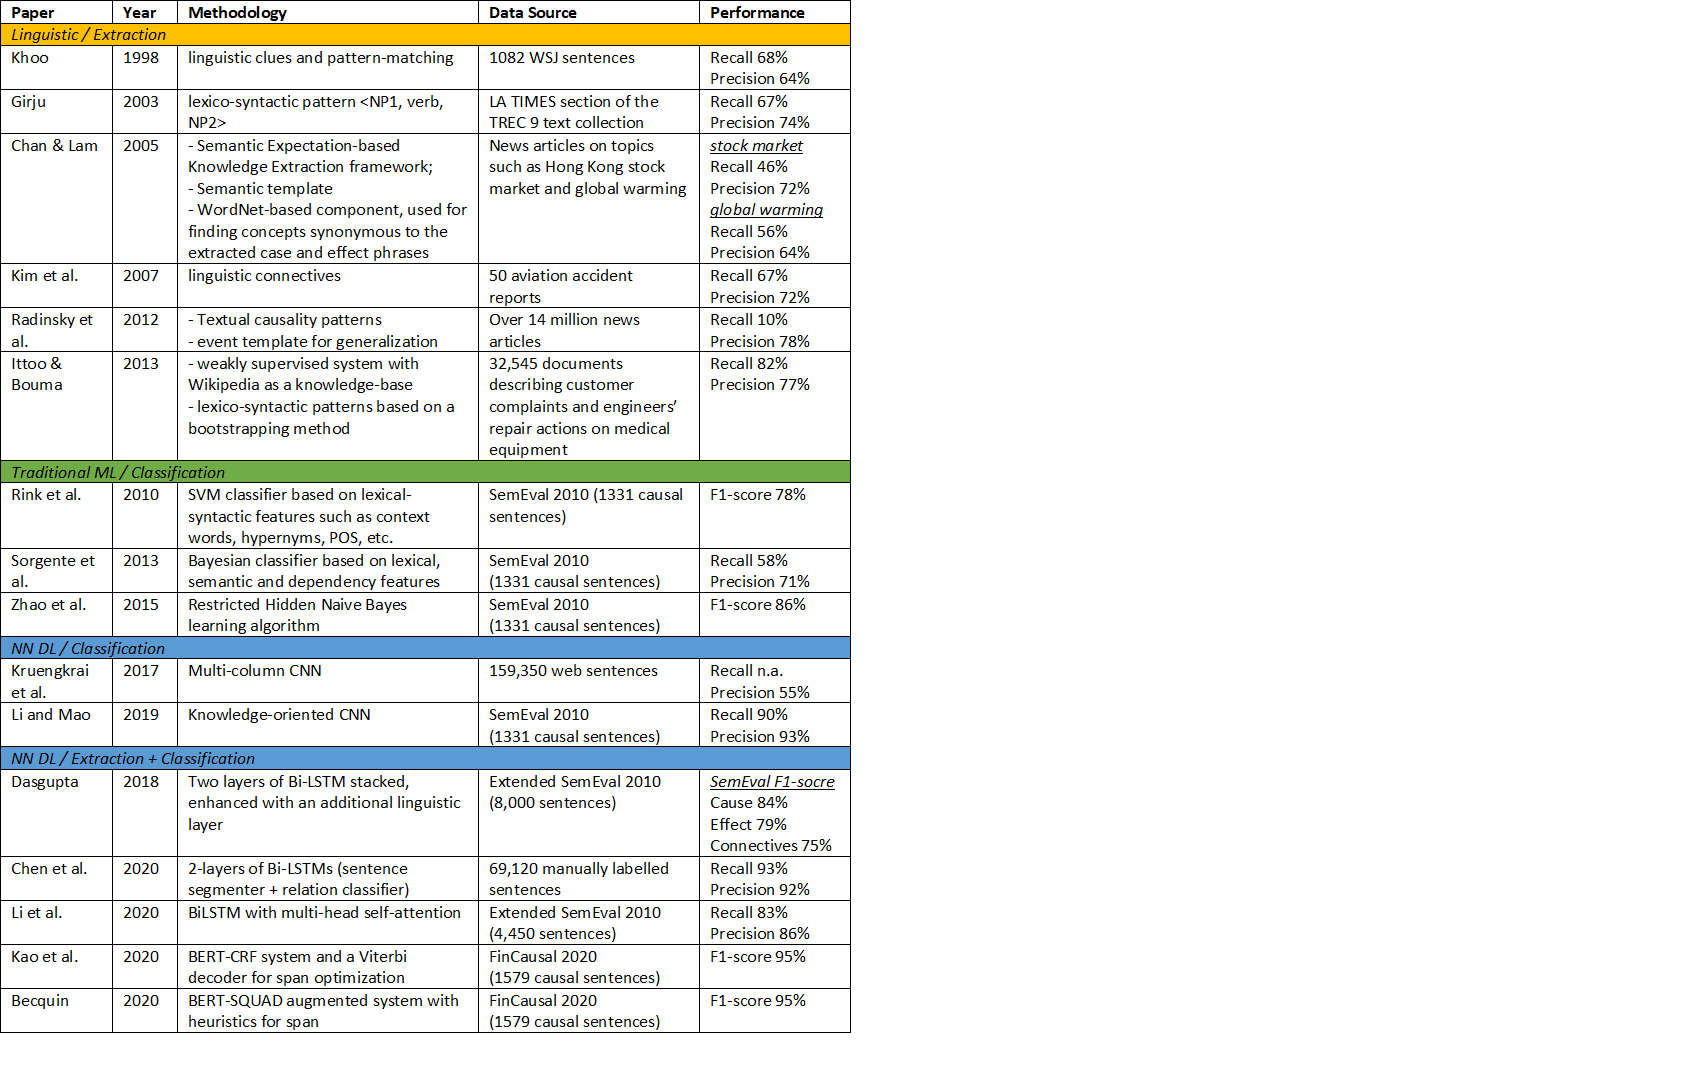
\includegraphics[scale=0.9]{figures/CE_papers.png}
  \caption{a summary table of all the papers relevant to causality extraction reviewed for this thesis.}
\end{figure}


\section{Exploratory Data Analysis on Raw MD\&A Texts} \label{appendix:EDA}

\begin{figure}
    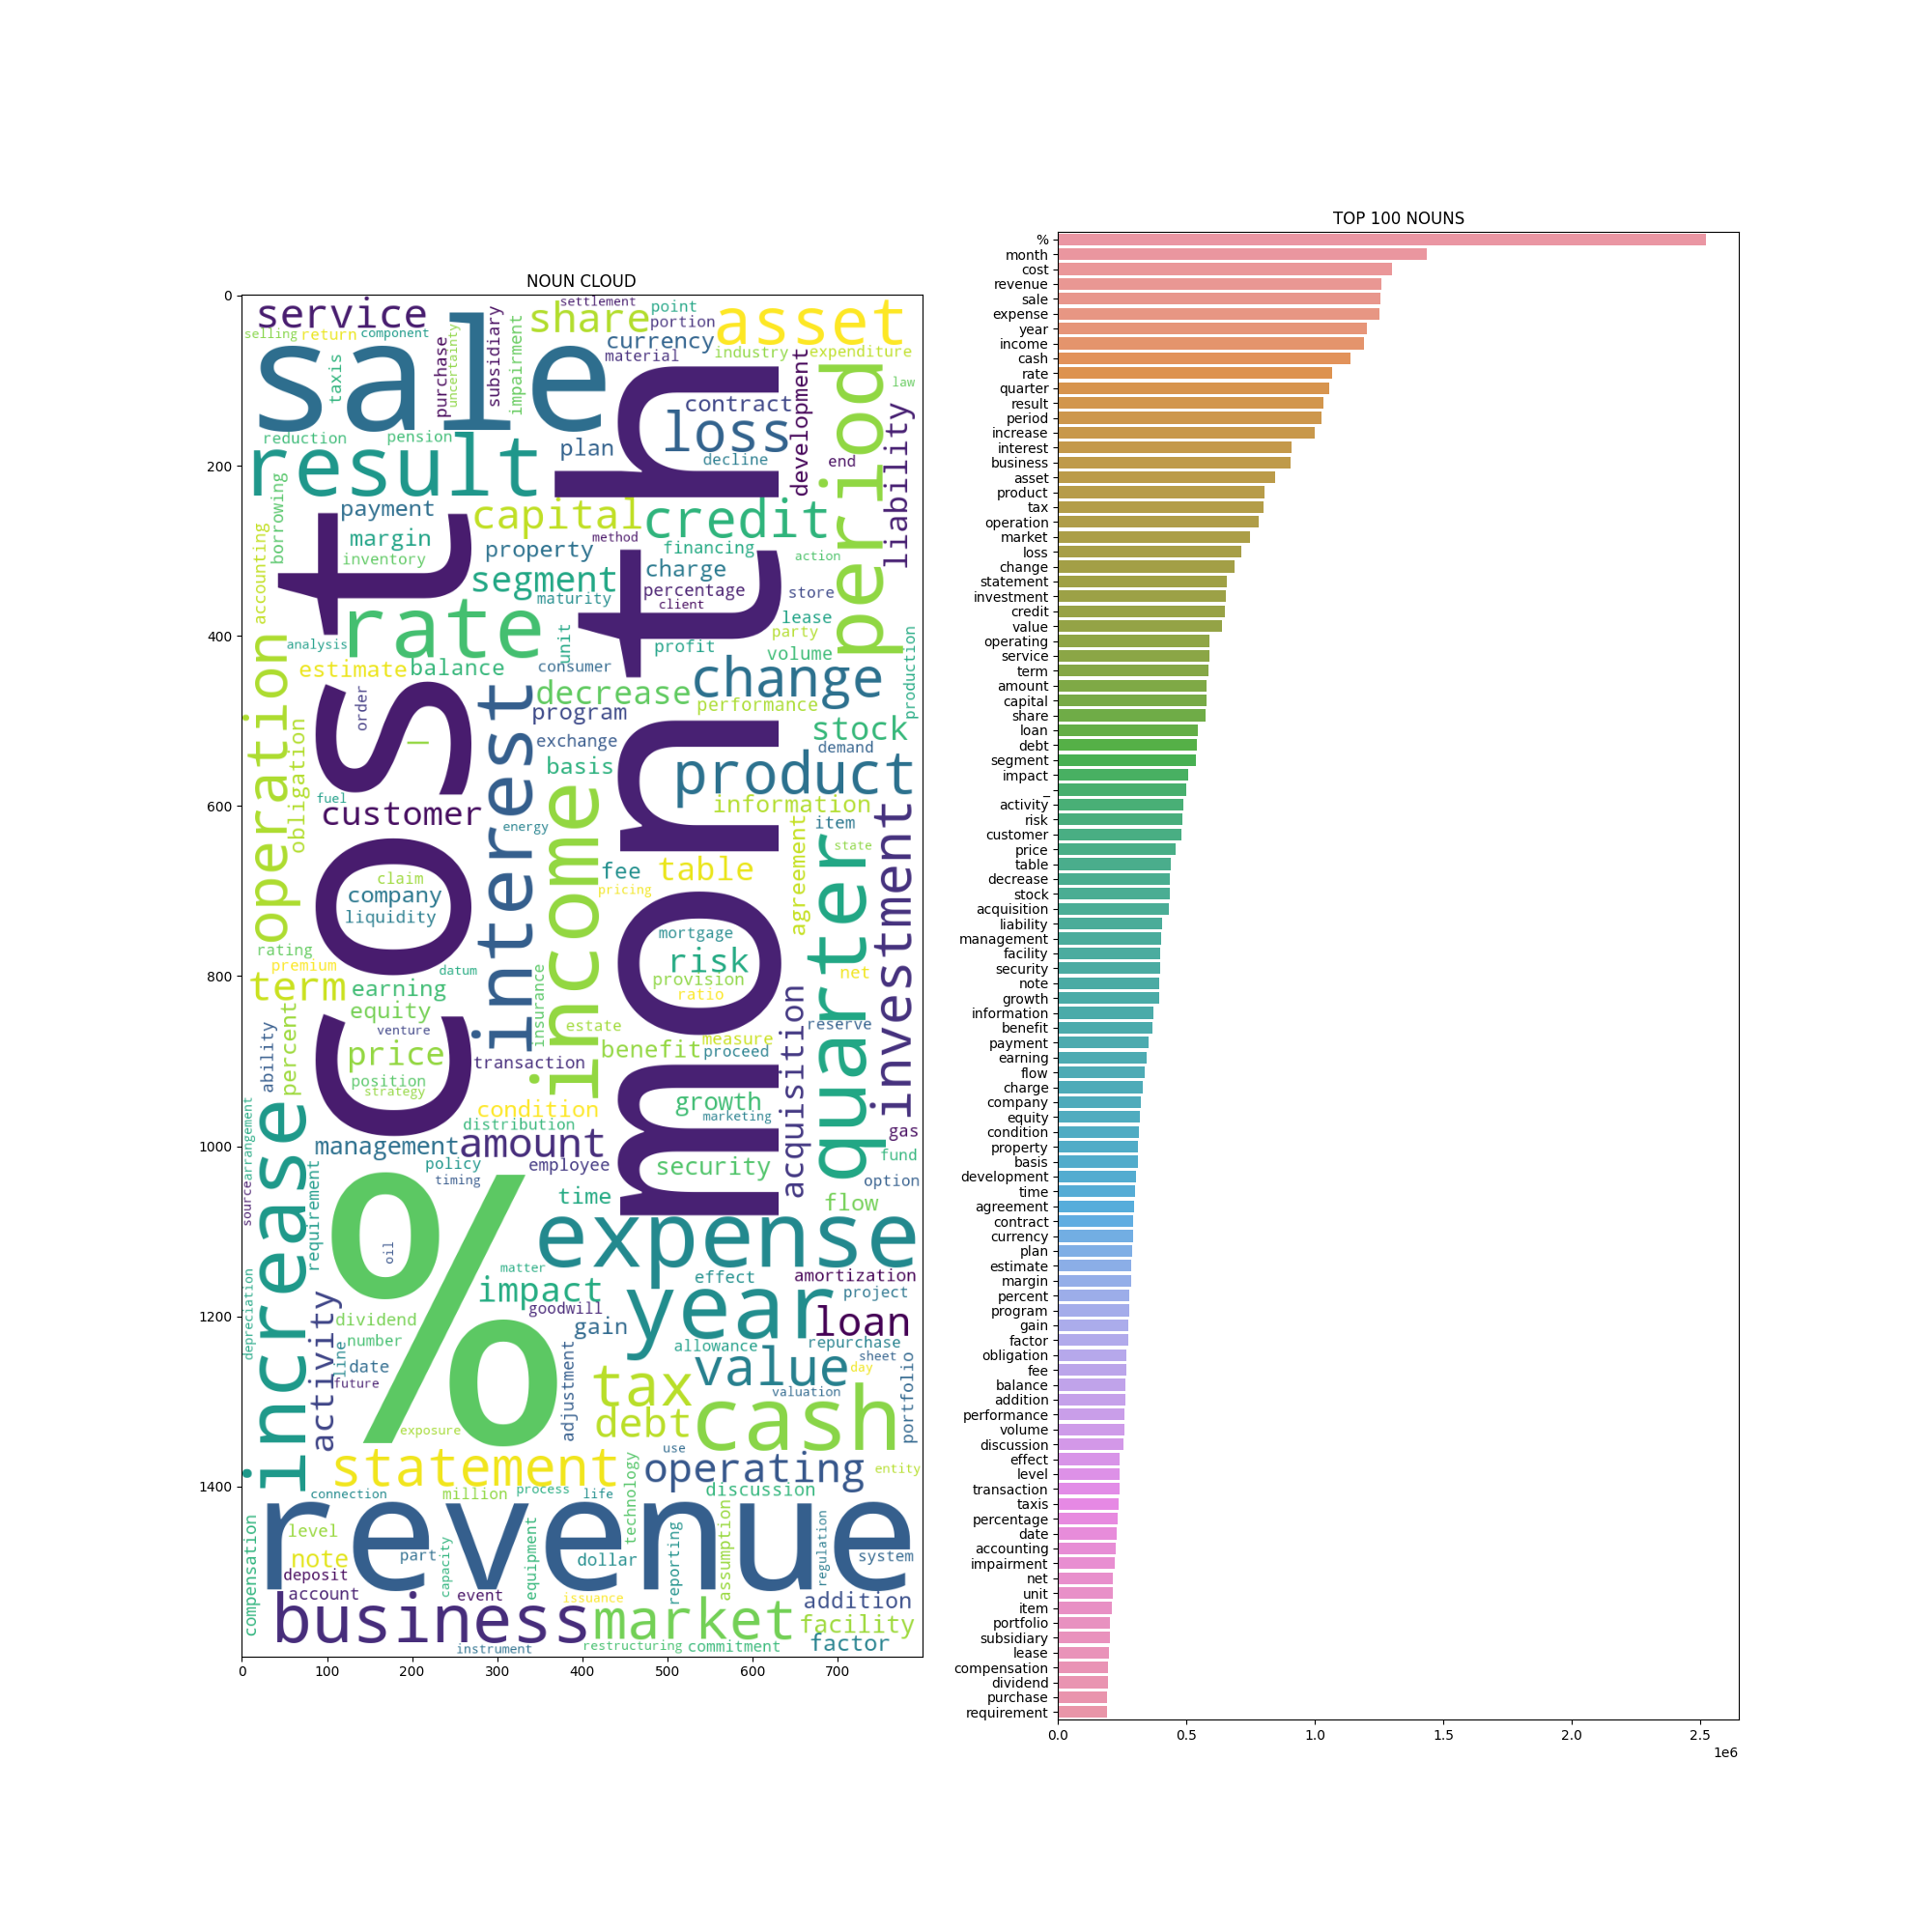
\includegraphics[width=\textwidth] {figures/NOUN_top100_figure.png}
    \caption{Word Cloud of Top 100 Nouns}
    \label{fig:NOUN}
\end{figure}

\begin{figure}[!tbp]
    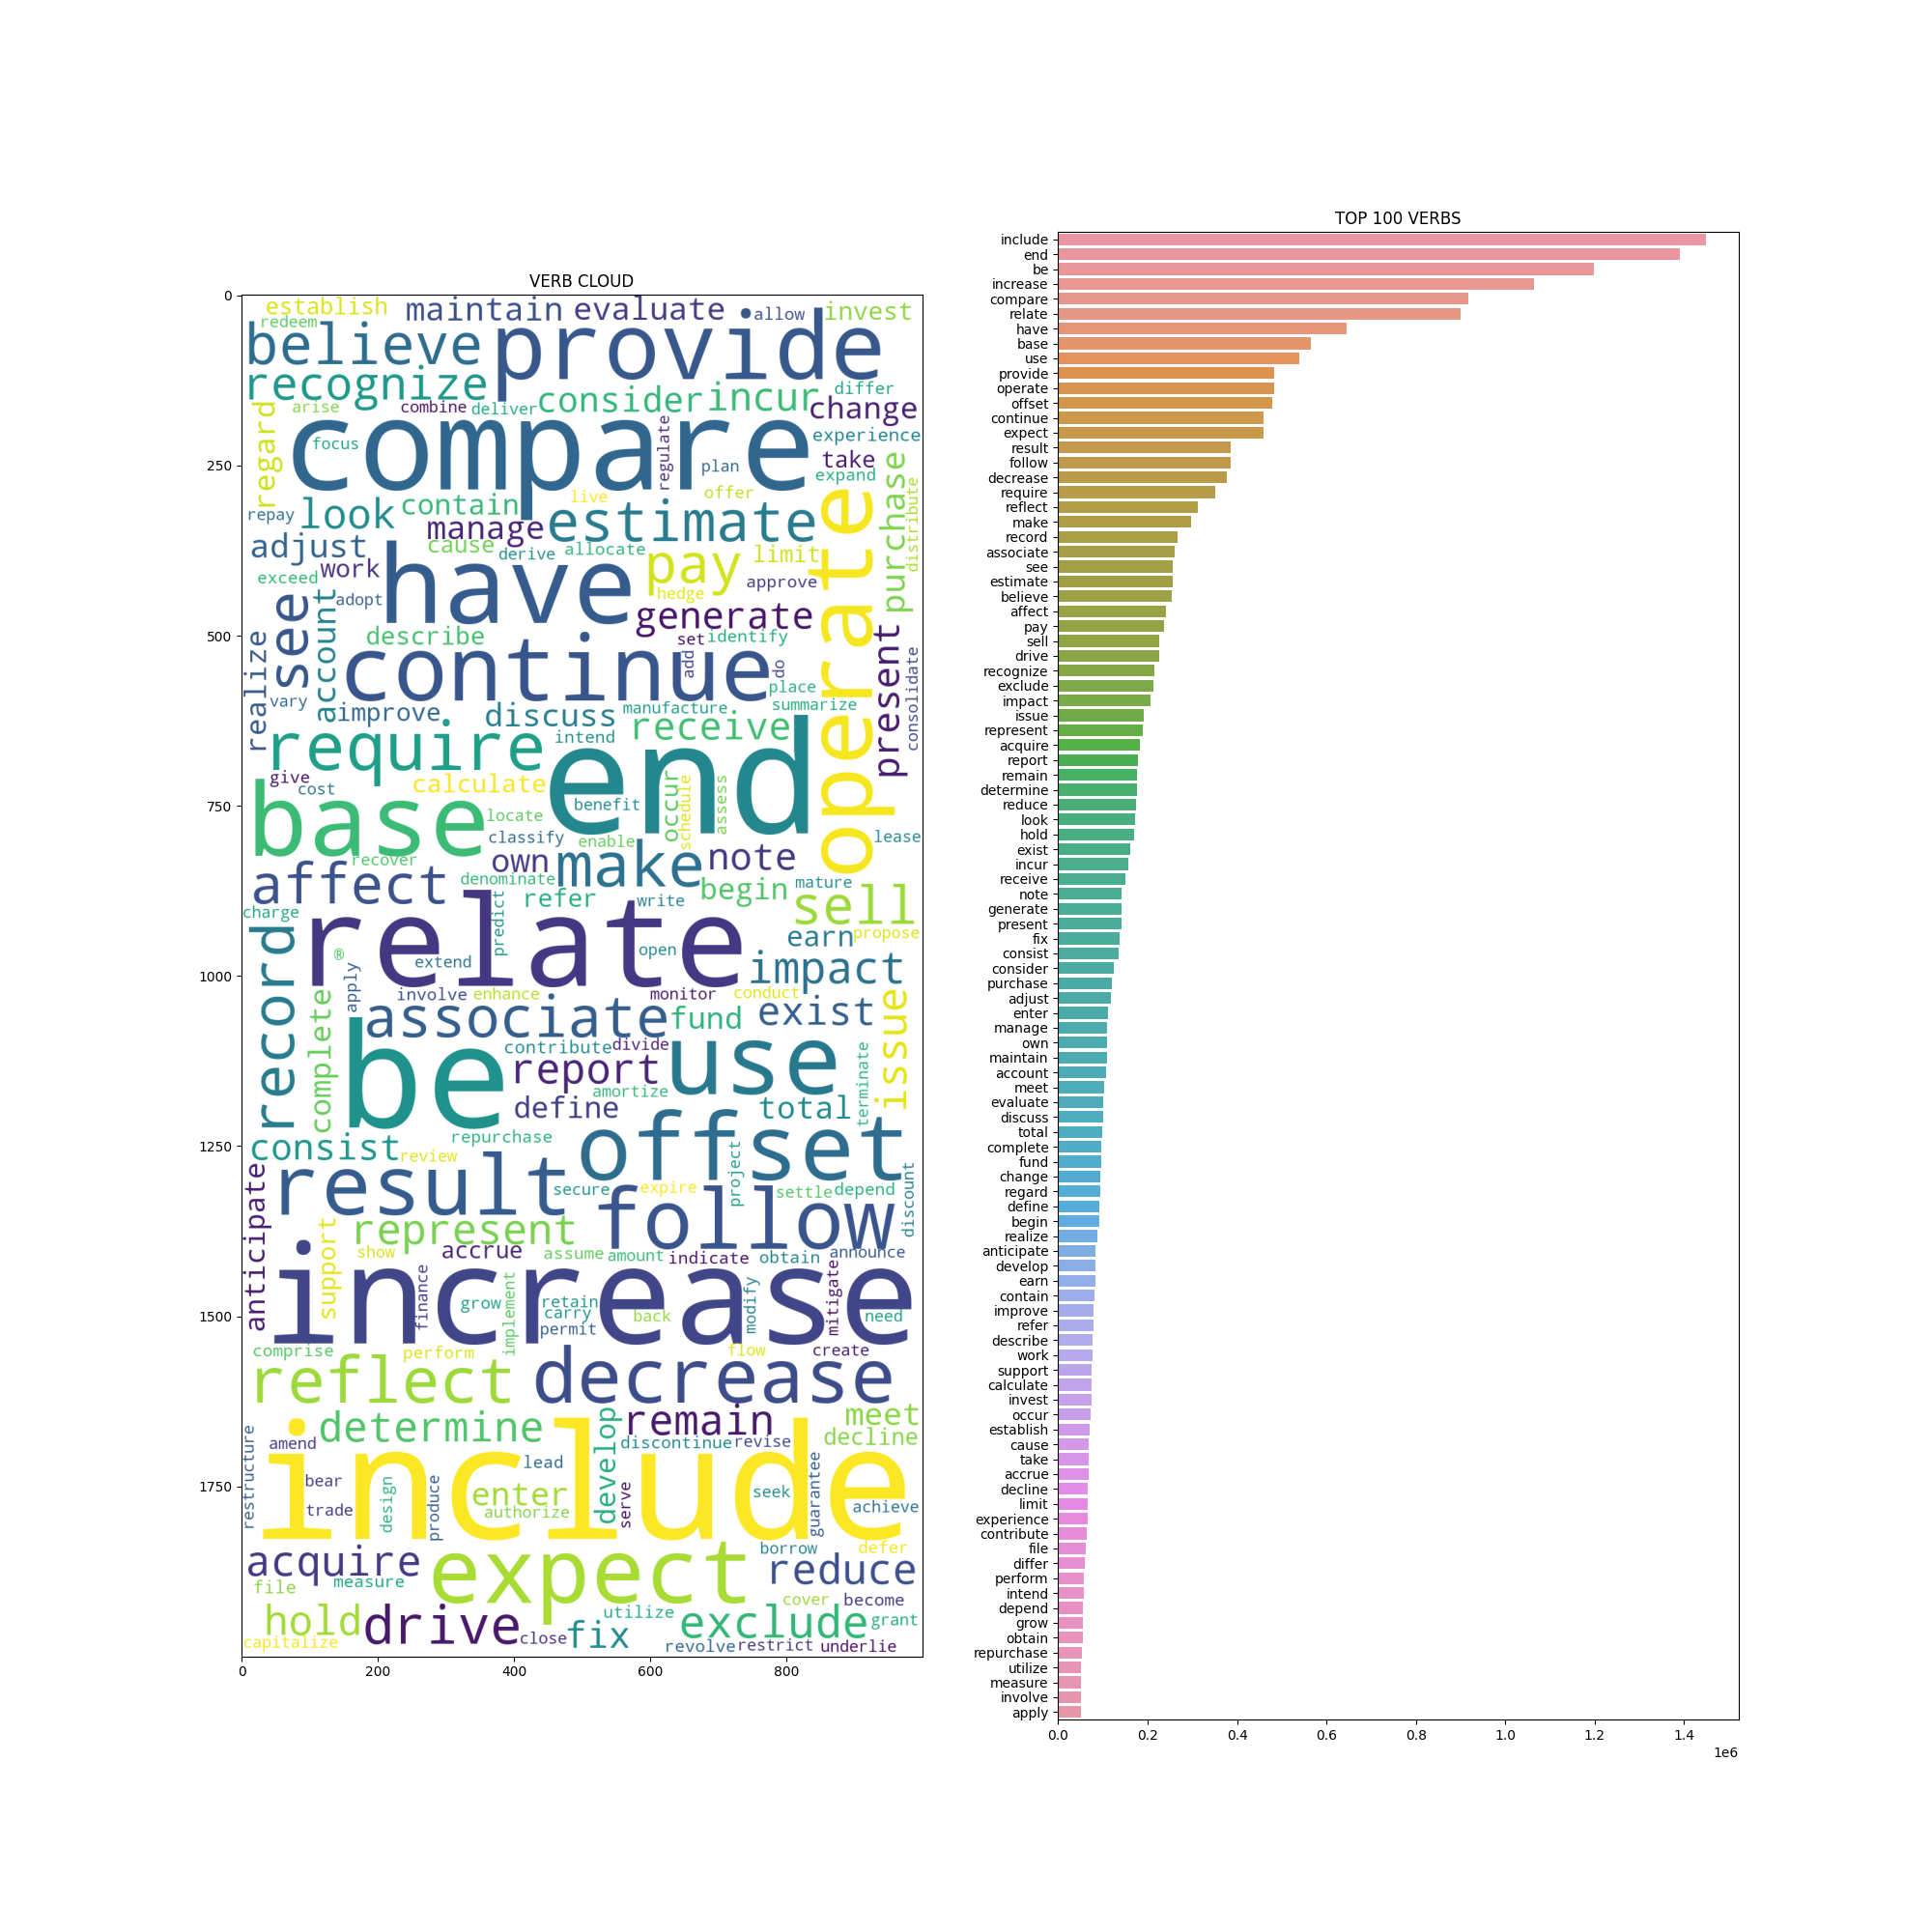
\includegraphics[width=\textwidth]{figures/VERB_top100_figure.png}
    \caption{Woud Cloud of Top 100 Verbs}
    \label{fig:VERB}
\end{figure}



\newpage

% References (Literaturverzeichnis):
% a) Style (with abbreviations: use alpha):
% see https://de.wikibooks.org/wiki/LaTeX-W%C3%B6rterbuch:_bibliographystyle
% for the different formats and styles
\bibliographystyle{ieeetr} %{apalike}

% b) The File:
\bibliography{references}

\end{document}
